%% ----------------------------------------------------------------
%% Thesis.tex -- MAIN FILE (the one that you compile with LaTeX)
%% ---------------------------------------------------------------- 

% Set up the document
\documentclass[a4paper, 11pt, oneside]{Thesis}  % Use the "Thesis" style, based on the ECS Thesis style by Steve Gunn
\graphicspath{Figures/}  % Location of the graphics files (set up for graphics to be in PDF format)

% Include any extra LaTeX packages required
\usepackage[square, numbers, comma, sort&compress]{natbib}  % Use the "Natbib" style for the references in the Bibliography
\usepackage{verbatim}  % Needed for the "comment" environment to make LaTeX comments
\usepackage{vector}  % Allows "\bvec{}" and "\buvec{}" for "blackboard" style bold vectors in maths
\usepackage{multirow}
\usepackage{hyperref}
\usepackage[table,xcdraw]{xcolor}
\hypersetup{urlcolor=blue, colorlinks=true}  % Colours hyperlinks in blue, but this can be distracting if there are many links.
\usepackage[font=small,labelfont=bf,
justification=justified,
format=plain]{caption} % 'format=plain' avoids hanging indentation

%% ----------------------------------------------------------------
\begin{document}
\frontmatter      % Begin Roman style (i, ii, iii, iv...) page numbering

% Set up the Title Page
\title  {Rejection Option in Pattern Recognition Problem - Selected Issues}
\authors  {\texorpdfstring
            {\href{waszkiewiczp@student.mini.pw.edu.pl}{Piotr Waszkiewicz}}
            {Piotr Waszkiewicz}
            }
\addresses  {\groupname\\\deptname\\\univname}  % Do not change this here, instead these must be set in the "Thesis.cls" file, please look through it instead
\date       {\today}
\subject    {}
\keywords   {}

\maketitle
%% ----------------------------------------------------------------

\setstretch{1.3}  % It is better to have smaller font and larger line spacing than the other way round

% Define the page headers using the FancyHdr package and set up for one-sided printing
\fancyhead{}  % Clears all page headers and footers
\rhead{\thepage}  % Sets the right side header to show the page number
\lhead{}  % Clears the left side page header

\pagestyle{fancy}  % Finally, use the "fancy" page style to implement the FancyHdr headers

%% ----------------------------------------------------------------
% Declaration Page required for the Thesis, your institution may give you a different text to place here
\Declaration{

\addtocontents{toc}{\vspace{1em}}  % Add a gap in the Contents, for aesthetics

I, Piotr Waszkiewicz, declare that this thesis titled, `Rejection Option in Pattern Recognition Problem - Selected Issues' and the work presented in it are my own. I confirm that:

\begin{itemize} 
\item[\tiny{$\blacksquare$}] This work was done wholly or mainly while in candidature for a research degree at this University.
 
\item[\tiny{$\blacksquare$}] Where any part of this thesis has previously been submitted for a degree or any other qualification at this University or any other institution, this has been clearly stated.
 
\item[\tiny{$\blacksquare$}] Where I have consulted the published work of others, this is always clearly attributed.
 
\item[\tiny{$\blacksquare$}] Where I have quoted from the work of others, the source is always given. With the exception of such quotations, this thesis is entirely my own work.
 
\item[\tiny{$\blacksquare$}] I have acknowledged all main sources of help.
 
\item[\tiny{$\blacksquare$}] Where the thesis is based on work done by myself jointly with others, I have made clear exactly what was done by others and what I have contributed myself.
\\
\end{itemize}
 
 
Signed:\\
\rule[1em]{25em}{0.5pt}  % This prints a line for the signature
 
Date:\\
\rule[1em]{25em}{0.5pt}  % This prints a line to write the date
}
\clearpage  % Declaration ended, now start a new page

%% ----------------------------------------------------------------
% The "Funny Quote Page"
% \pagestyle{empty}  % No headers or footers for the following pages

% \null\vfill
% Now comes the "Funny Quote", written in italics
% \textit{``Write a funny quote here.''}

% \begin{flushright}
% If the quote is taken from someone, their name goes here
% \end{flushright}

% \vfill\vfill\vfill\vfill\vfill\vfill\null
% \clearpage  % Funny Quote page ended, start a new page
%% ----------------------------------------------------------------

% The Abstract Page
\addtotoc{Abstract}  % Add the "Abstract" page entry to the Contents
\abstract{
\addtocontents{toc}{\vspace{1em}}  % Add a gap in the Contents, for aesthetics

An analysis of the presented study seeks a solution to a common problem in a classification issue, which is detecting and rejecting data not suited for classification. Contaminated data that emerges from noisy environment can lead to a situation in which even well trained models yield bad results. This is a serious problem for processes that rely on a classifiers' efficiency in which rejecting received data is more acceptable than classifying it wrongly, e.g. tumor detection algorithm should refuse to make medical evaluation of provided image if it is too blurry rather than trying to guess patient's health condition. \\

Although artificial intelligence gained much importance and is used in many aspects of humans life (even outside of pure scientific fields), there's still a need for newer approaches and methods. Commonly used algorithms and models change very frequently as new problems arise. Study presented in this thesis introduces modifications to some of the oldest and well known techniques and tries to combine them in order to create tools with much higher capabilities.

}

\clearpage  % Abstract ended, start a new page
%% ----------------------------------------------------------------

\setstretch{1.3}  % Reset the line-spacing to 1.3 for body text (if it has changed)

% The Acknowledgements page, for thanking everyone
\acknowledgements{
\addtocontents{toc}{\vspace{1em}}  % Add a gap in the Contents, for aesthetics

The acknowledgements and the people to thank go here, don't forget to include your project advisor\ldots

}
\clearpage  % End of the Acknowledgements
%% ----------------------------------------------------------------

\pagestyle{fancy}  %The page style headers have been "empty" all this time, now use the "fancy" headers as defined before to bring them back


%% ----------------------------------------------------------------
\lhead{\emph{Contents}}  % Set the left side page header to "Contents"
\tableofcontents  % Write out the Table of Contents

%% ----------------------------------------------------------------
\lhead{\emph{List of Figures}}  % Set the left side page header to "List if Figures"
\listoffigures  % Write out the List of Figures

%% ----------------------------------------------------------------
\lhead{\emph{List of Tables}}  % Set the left side page header to "List of Tables"
\listoftables  % Write out the List of Tables

%% ----------------------------------------------------------------
\setstretch{1.5}  % Set the line spacing to 1.5, this makes the following tables easier to read
% \clearpage  % Start a new page
% \lhead{\emph{Abbreviations}}  % Set the left side page header to "Abbreviations"
% \listofsymbols{ll}  % Include a list of Abbreviations (a table of two columns)
% {
% \textbf{Acronym} & \textbf{W}hat (it) \textbf{S}tands \textbf{F}or \\
% \textbf{LAH} & \textbf{L}ist \textbf{A}bbreviations \textbf{H}ere \\
% }

%% ----------------------------------------------------------------
% \clearpage  % Start a new page
% \lhead{\emph{Physical Constants}}  % Set the left side page header to "Physical Constants"
% \listofconstants{lrcl}  % Include a list of Physical Constants (a four column table)
% {
% Constant Name & Symbol & = & Constant Value (with units) \\
% Speed of Light & $c$ & $=$ & $2.997\ 924\ 58\times10^{8}\ \mbox{ms}^{-\mbox{s}}$ (exact)\\
% }

%% ----------------------------------------------------------------
% \clearpage  %Start a new page
% \lhead{\emph{Symbols}}  % Set the left side page header to "Symbols"
% \listofnomenclature{lll}  % Include a list of Symbols (a three column table)
% {
% symbol & name & unit \\
% $a$ & distance & m \\
% $P$ & power & W (Js$^{-1}$) \\
% & & \\ % Gap to separate the Roman symbols from the Greek
% $\omega$ & angular frequency & rads$^{-1}$ \\
% }
%% ----------------------------------------------------------------
% End of the pre-able, contents and lists of things
% Begin the Dedication page

% \setstretch{1.3}  % Return the line spacing back to 1.3
% \pagestyle{empty}  % Page style needs to be empty for this page
% \dedicatory{For/Dedicated to/To my\ldots}
% \addtocontents{toc}{\vspace{2em}}  % Add a gap in the Contents, for aesthetics


%% ----------------------------------------------------------------
\mainmatter	  % Begin normal, numeric (1,2,3...) page numbering
\pagestyle{fancy}  % Return the page headers back to the "fancy" style

% Include the chapters of the thesis, as separate files
% Just uncomment the lines as you write the chapters

\lhead{\emph{Introduction}}
\chapter{Introduction}

Study presented in this paper tries to combine few selected classifiers in such way that will empower them to gain rejection capabilities. The main goal is to come up with a model which structure allows to reject patterns that are outside of native elements classes' scope without any prior knowledge about such patterns. Those outliers, denoted as foreign elements, are very common in real life situations when dealing with noisy, erroneous or unknown measurements. The main drawback of commonly used classifiers is their inability to reject foreign elements without any knowledge about them. Classifiers such as SVM, random forest or kNN (described better in Chapter \ref{common_classifiers}) must always put presented pattern to one of the classes they were trained on. This  requirement to always classify provided pattern to one of the classes their were trained on forces inclusion of foreign elements within training sets if there's a need to reject certain elements. Although not impossible, this approach is quite impractical as most of the time there are just too many possible cases of foreign elements. This paper tries to find solution to this presented problem.

The document is structured as follows: the first chapter introduces reader to the commonly used, well-known classifiers, describing their structures and briefly explaining the way they work. The next chapter covers quality measurements which help in evaluating proposed solutions and their results. Next, the datasets used during testing process are described. The following chapters present proposed classifier structures with rejection option, explaining the main ideas behind them and comparing their results achieved on provided data. 

 % Introduction

\lhead{\emph{Common Classifiers}}

\chapter{Common Classifiers}
\label{common_classifiers}

The task of classification aims at categorising unknown elements to their appropriate groups. The procedure is based on quantifiable characteristics obtained from the source signal. Those characteristics, i.e.~features, are gathered in a~feature vector (a~vector of independent variables) and each pattern is described with one feature vector. It is expected that patterns accounted to the same category are in a~relationship with one another. In other words, subjects and objects of knowledge accounted to the same category are expected to be in some sense similar. There are many mathematical models that can be used as classifiers, such as SVM, random forest, kNN, regression models, or Neural Networks. Their main disadvantage lies in their need to be trained prior to usage, which makes them unable to recognize elements from a~new class, not present during the training process. This behaviour can be especially troublesome in an unstable, noisy environment, where patterns sent for classification can be corrupted, distorted or otherwise indistinguishable.

\section{Implementation}

Implementations of the common classifiers described in this chapter were taken from scikit-learn\footnote{scikit-learn webpage: \href{http://scikit-learn.org/}{http://scikit-learn.org}} Python library\cite{Pedregosa2011}. It is a popular, open source project using BSD license and built on NumPy\footnote{NumPy webpage: \href{http://www.numpy.org/}{http://www.numpy.org}}, SciPy\footnote{SciPy webpage: \href{https://www.scipy.org/}{https://www.scipy.org}} and matplotlib libraries. The project was started in 2007 by David Cournapeau as a Google Summer of Code project and is currently maintained by a team of volunteers. The library contains implementations of many algorithms to be used, among others, in classification, regression, clustering, dimensionality reduction and preprocessing problems.

\section{kNN}

The k-Nearest Neighbours algorithm, denoted as kNN, is an example of a~``lazy classifier'', where the entire training dataset is the model. There is no typical model building phase, hence the name. Class membership is determined based on class labels encountered in $k$~closest observations in the training dataset,~\cite{Altman1992}. In a~typical application, the only choice that the model designer has to make is selection of $k$~and distance metrics. Both are often determined experimentally with a~help of supervised learning procedures. Example of area coverage for three classes used in kNN classification issue can be seen in Figure \ref{fig:knn_schema}.

The kNN classifier implementation available within scikit-learn package allows to make adjustments to certain parameters that are crucial in classification issue:
\begin{itemize}
	\item $n\_neighbors$ - corresponds to the $k$ value, determines number of nearest points used to classify pattern
	\item $metric$ - the distance metric to use for the tree
\end{itemize}

\begin{figure}[htp]
	\centering
	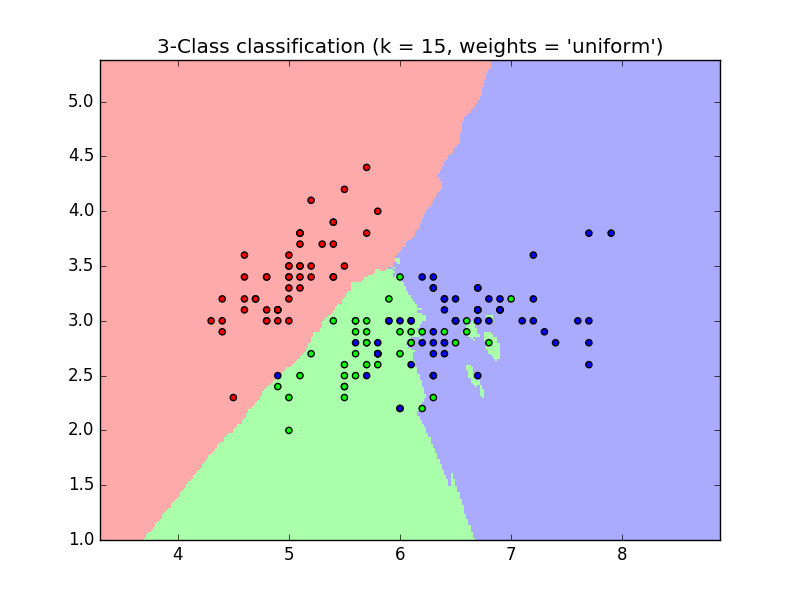
\includegraphics[width=0.7\textwidth]{Figures/knn_schema.png}
	\caption{Visualization of area coverage of three different class membership for kNN classifier with k=15, using euclidean metric. Image taken from \cite{Scikit-Learn_Website}}
	\label{fig:knn_schema}\vspace{-3pt}
\end{figure}

\section{SVM}

Support Vector Machines (SVM) are a~collection of supervised learning methods used for classification, regression and outliers detection. The SVM algorithm relies on a~construction of hyperplane with a~maximal margin that separates patterns of two classes~\cite{CortesVapnik1995}. Creation of the hyper-plane that has the largest distance to the nearest training data points of any class (so-called functional margin) is important since, in general, the larger the margin the lower the generalization error of the classifier.

In SVM's mathematical definition the two classes' labels are denoted as -1 and 1. When treating elements from those sets as points of the Euclidean space $\mathbb{R}^{n}$ (or vectors of this space) the SVM training can be seen as the problem of finding the maximum-margin hyperplane that divides those samples. This issue can be described by formula: \[ w * x - b = 0 \] where $w, x \in \mathbb{R}^{n}, b \in \mathbb{R}$. The $x_{i}$ vectors are samples from the training set, and $w$ is a normal vector to the hyperplane, obtained as a linear combination of those training vectors that lie at borders of the margin: \[ w = \Sigma_{i}\alpha_{i}x_{i} \] Those of the training vectors $x_{i}$ that satisfy the following condition: \[ y_{i}(x * x_{i} - b) = 1\] are called support vectors, and have their corresponding $\alpha_{i} \neq 0$. The $y_{i} \in {-1, 1}$ corresponds to the class labels that training data consists of. The linear decision function used for classifying patterns is expressed as follows: \[I(x) = sgn(\Sigma\alpha_{i}x_{i} * x - b)\] where $\alpha_{i}x_{i} = w_{i}$. SVM efficiency can be enhanced by using different kernel functions which help in solving non-linearly-separable problems. The generalized decision function using kernel function $K$: \[I(x) = sgn(\Sigma\alpha_{i}K(x_{i},x) - b)\]

\begin{figure}[htp]
	\centering
	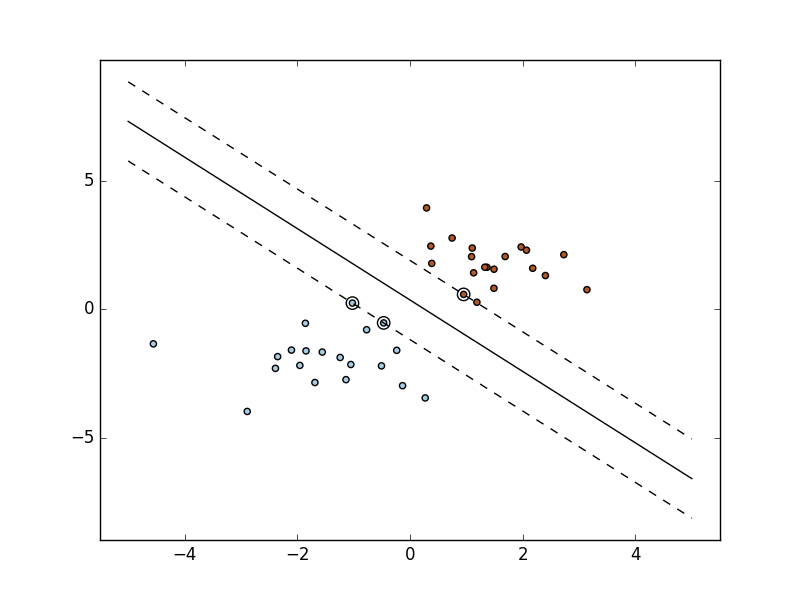
\includegraphics[width=0.7\textwidth]{Figures/svm_hyperplane_margin.png}
	\caption{SVM hyperplane construction with the biggest possible margin for training dataset. Image taken from \cite{Scikit-Learn_Website}}
	\label{fig:svm_hyperplane_margin}\vspace{-3pt}
\end{figure}


\begin{figure}[htp]
	\centering
	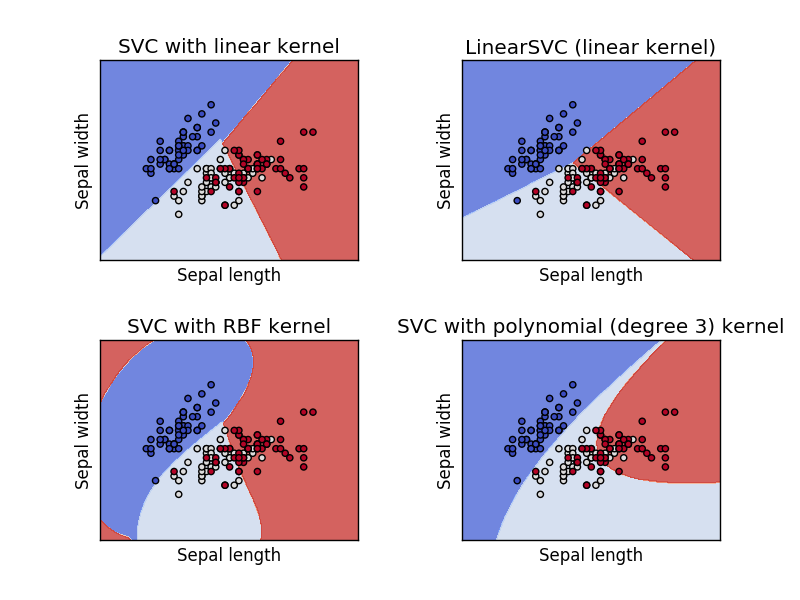
\includegraphics[width=1.0\textwidth]{Figures/svm_kernel_functions.png}
	\caption{Different class area coverages resulting from usage of different kernel functions. Image taken from \cite{Scikit-Learn_Website}}
	\label{fig:svm_kernel_functions}\vspace{-3pt}
\end{figure}

SVMs are effective in high-dimensional spaces, memory efficient, and quite versatile because of the many kernel functions that can be specified for the decision function. Implementation available as part of scikit-learn package lets user specify and tweak many aspects of classifier such as:

\begin{itemize}
	\item $C$ - penalty parameter C of the error term, used to regularize the estimation. If dealing with noisy observations it's recommended to decrease its value
	\item $kernel$ - kernel type used in the algorithm, in this paper one of "poly" or "rbf" values are used. "poly" stands for polynomial kernel using following equation $(\gamma \langle x, x' \rangle + r)^{d}$ (where d is function degree, with default value 3), "rbf" is an acronym for radial basis function with given equation $exp(-\gamma|x - x'|^{2})$
	\item $gamma$ - kernel coefficient for "rbf", "poly" types as can be seen it the kernel equations
	\item $degree$ - degree of the polynomial kernel function
\end{itemize}

It is worth noting though that in some cases, where the number of features is much greater than the number of samples, using support vector machines can give poor results, and is not cost-efficient when calculating probability estimates. 

\section{Random Forest}

Random forest is a~popular ensemble method. The main principle behind ensemble methods, in general, is that a~group of ``weak learners'' can come together to form a~``strong learner''. In the random forest algorithm~\cite{Breiman2001} the weak learners are decision trees, which are used to predict class labels. A decision tree is a decision support tool that uses a tree-like graph for classification issue. Each graph node performs a test on an attribute of the provided pattern and sends it to its child node via a branch that represents the outcome of the test. Each leaf in a decision tree represents a certain class label. In other words for a~feature vector representing one pattern a~decision tree calculates its class label by dividing value space into two or more subspaces. More precisely, an input data is entered at the top of the tree and as it traverses down the tree the data gets bucketed into smaller subsets. There are many advantages of using decision trees. Their results are easy to interpret and visualize in form of a graph, they can handle multi class classification problems and perform well even if its assumptions are somewhat violated by the true model from which the data were generated. On the other hand, the main drawbacks connected to their usage consist of overfitting problem caused by creating too complex trees on a very complicated data, and instability caused by small variations in the data that might result in a completely different tree being generated. That last problem is easily mitigated by ensembling set of decision trees into a random forest. 

\begin{figure}[htp]
	\centering
	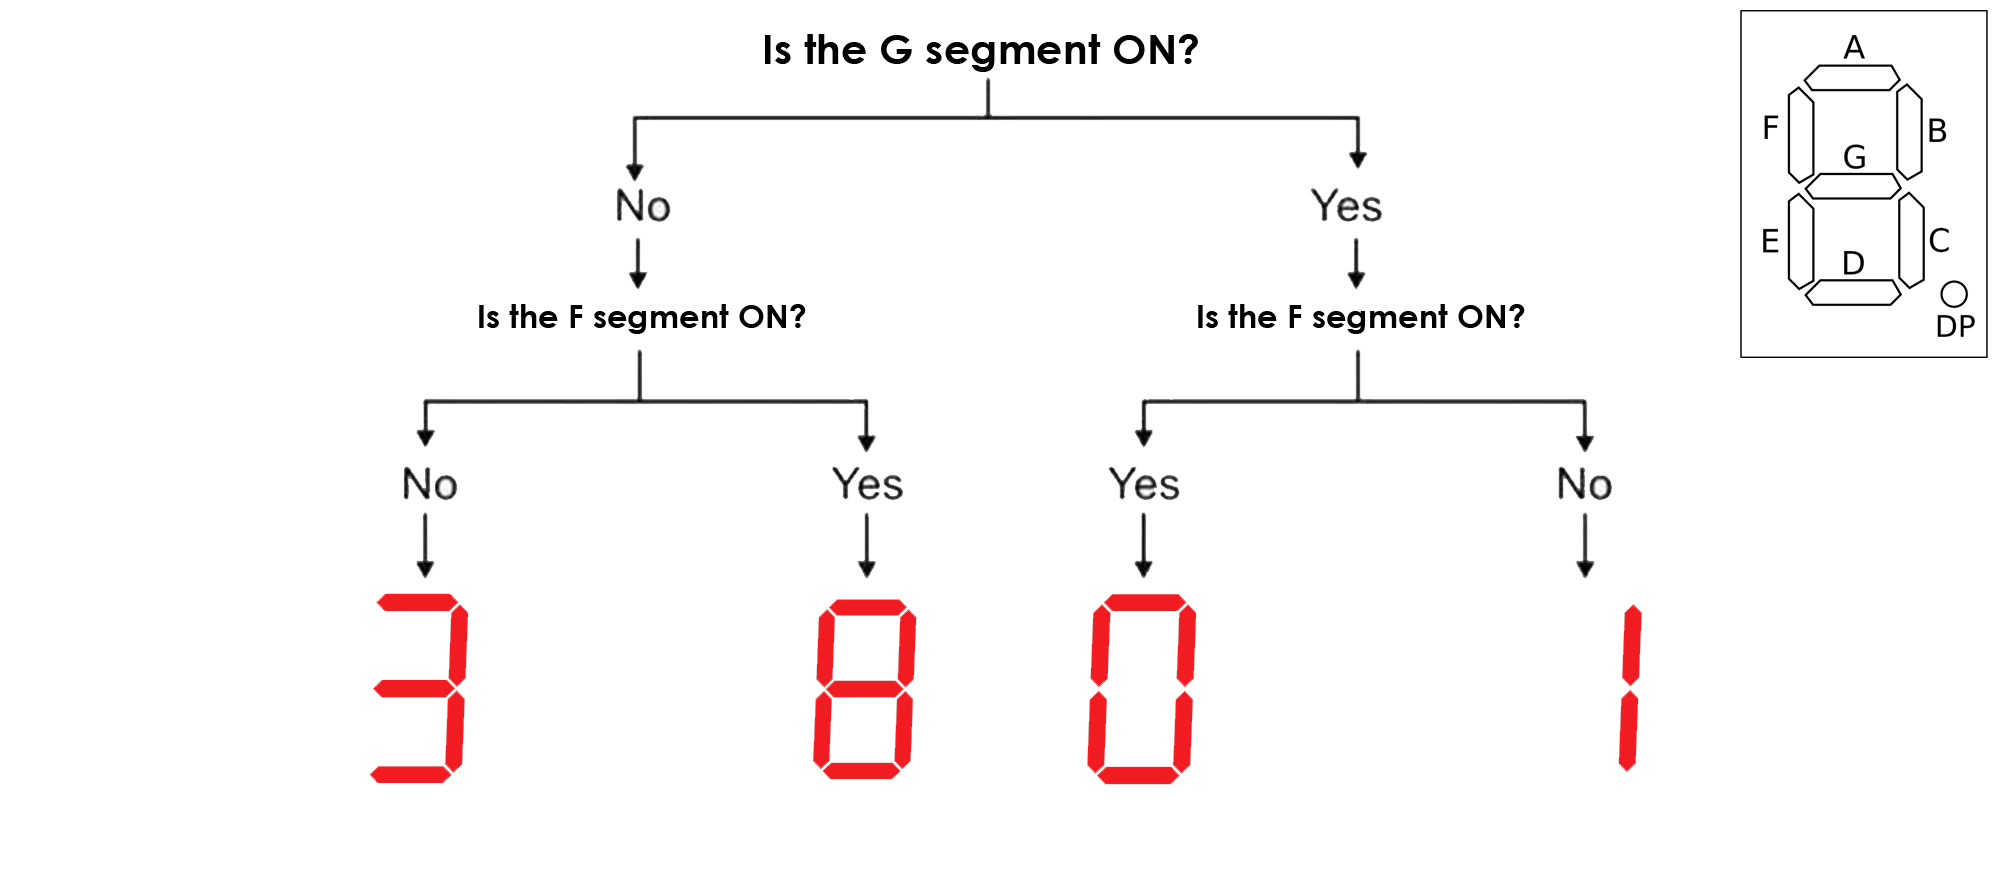
\includegraphics[width=0.8\textwidth]{Figures/rf_visualization_funny.jpg}
	\caption{A funny example of a decision tree}
	\label{fig:rf_visualization_funny}\vspace{-3pt}
\end{figure}

In the random forest a~large number of classification trees is formed, which altogether serve as a~classifier. In order to grow each tree, a~random selection of rows from the training set is drawn. Random sampling with replacement is also called bootstrap sampling. In addition, when constructing trees for a~random forest at each node $m$~variables out of the set of all input variables are randomly selected, and the best split on these $m$~is used to split the node. After a~relatively large number of trees is generated, they vote for the most popular class. Some of the parameters used for improving classification rates that are available within scikit-learn package random forest implementation:

\begin{itemize}
	\item $n\_estimators$ - determines number of trees used by random forest in the algorithm
	\item $max\_depth$ - the maximum depth of each tree in the forest
	\item $max\_features$ - the number of features to consider when looking for the best split
	\item $min\_samples\_leaf$ - the minimum number of samples required to be at a leaf node
\end{itemize}

Random forests join few important benefits: (a)~they are relatively prone to the influence of outliers, (b)~they have an embedded ability of feature selection, (c)~they are prone to missing values, and (d)~they are prone to over-fitting.

\begin{figure}[htp]
	\centering
	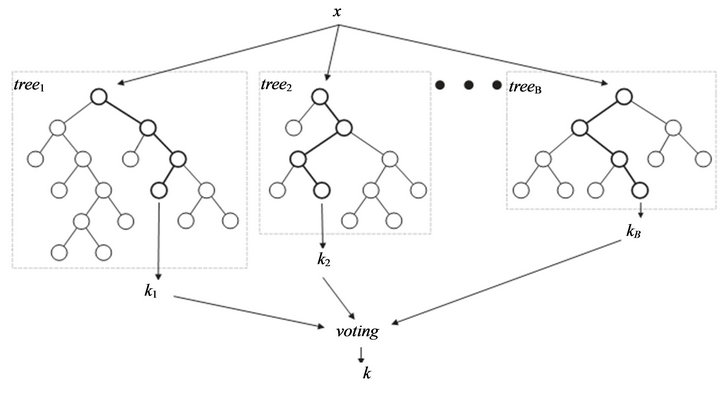
\includegraphics[width=1.0\textwidth]{Figures/rf_visualization.jpg}
	\caption{Visualization of a random forest consisting of $B$ different decision trees}
	\label{fig:rf_visualization}\vspace{-3pt}
\end{figure} % Background Theory 

\lhead{\emph{Quality Evaluation}}
\chapter{Quality Evaluation} \label{quality_measures}

In order to evaluate the quality of the proposed methods a~set of measures is used, described below and in Table~\ref{tab:measures}.
\begin{itemize}
	\item \emph{Correctly Classified} is the number of native patterns classified as native with a~correct class label.
	\item \emph{True Positives} is the number of native patterns classified as native (no matter, into which native class).
	\item \emph{False Negatives} is the number of native patterns incorrectly classified as foreign.
	\item \emph{False Positives} is the number of foreign patterns incorrectly classified as native.
	\item \emph{True Negatives} is the number of foreign patterns correctly classified as foreign.
\end{itemize}  


\begin{table}[!h]
	\vspace{-6pt}
	\centering
	\caption{Quality measures for classification with rejection.}
	\vspace{-6pt}
	{\footnotesize
		\begin{tabular}{rclrcl}
			$\textnormal{Native Precision}$ &$=$& $\displaystyle\frac{\textnormal{TP}}{\textnormal{TP+FP}}$ & 
			$\textnormal{Accuracy}$ &$=$& $\displaystyle\frac{\textnormal{TP+TN}}{\textnormal{TP+FN+FP+TN}}$ \\
			&&&&&\vspace{-3pt}\\
			$\textnormal{Foreign Precision}$ &$=$& $\displaystyle\frac{\textnormal{TN}}{\textnormal{TN+FN}}$ &
			$\textnormal{Strict Accuracy}$ &$=$& $\displaystyle\frac{\textnormal{CC+TN}}{\textnormal{TP+FN+FP+TN}}$ \\
			&&&&&\vspace{-3pt}\\
			$\textnormal{Native Sensitivity}$ &$=$& $\displaystyle\frac{\textnormal{TP}}{\textnormal{TP+FN}}$ &
			$\textnormal{Fine Accuracy}$ &$=$& $\displaystyle\frac{\textnormal{CC}}{\textnormal{TP}}$ \\
			&&&&&\vspace{-3pt}\\
			$\textnormal{Foreign Sensitivity}$ &$=$& $\displaystyle\frac{\textnormal{TN}}{\textnormal{TN+FP}}$ &
			$\hspace{18pt}\textnormal{Strict Native Sensitivity}$ &$=$& $\displaystyle\frac{\textnormal{CC}}{\textnormal{TP+FN}}$\\
			&&&&&\vspace{-3pt}\\
			\multicolumn{6}{c}{$\textnormal{F--measure}=2\cdot\displaystyle\frac{\textnormal{Precision}\cdot\textnormal{Sensitivity}}{\textnormal{Precision}+\textnormal{Sensitivity}}$}
		\end{tabular}
	}
	\label{tab:measures}
	\vspace{-12pt}
\end{table} % Experimental Setup

\lhead{\emph{Datasets}}
\chapter{Datasets} \label{datasets}

All quality measures described in Chapter \ref{quality_measures} obtained and presented in this paper are calculated from classifiers' results for certain datasets. Those sets, referred to as native and foreign, are the result of applying feature-extraction function to images containing digits and letters. The original data comes from the well-known MNIST database\cite{MNIST}, which comprises the image files of handwritten upper-case letters, which have been size-normalized and centered in a fixed-size image. It is a good database for people who want to try learning techniques and pattern recognition methods on real-world data while spending minimal efforts on preprocessing and formatting.

\begin{figure}[htp]
	\centering
	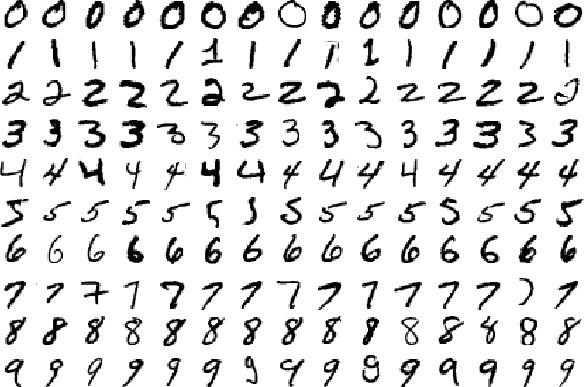
\includegraphics[width=0.7\textwidth]{Figures/mnistdigits.jpg}
	\caption{Visualization of scanned digits from MNIST database, image taken from \cite{Kuan_Hoong_Blog}}
	\label{fig:mnist_digits}\vspace{-3pt}
\end{figure}

The native set consists of 10,000 scanned digit images, with ten different classes one for every digit (0 - 9) and approximately 1000 samples for each class. This set is further divided into training and test sets in 7:3 ratio. The foreign set consists of 26,000 images of scanned letters and is not divided internally because it is used only in rejection option evaluation. All patterns within those two sets have been size-normalized and centred in a fixed-size image. Every pattern within those two datasets consists of 24 unique features that were extracted to ensure best classification capabilities. Examples of features are: maximum/position of maximum values of projections, histograms of projections, transitions, offsets; raw moments, central moments, Euler numbers etc.  % Dataset description

\lhead{\emph{Classifier Trees}}

\chapter{Classifier Trees}

Common classifiers described in the Chapter \ref{common_classifiers} return results in form of a class label that provided pattern was classified to. Such approach leaves no room for estimating class-belonging probabilities which, in return, results in inability to reject provided data, treating it as an outlier. By combining those classifiers and organising them in a complex structures it is possible to create objects with unique rejection capabilities in exchange for slightly increased pattern-processing time. This chapter describes such structures, shaped in form of binary trees.

\section{Balanced Tree}

\subsection{Structure}

The main idea behind Balanced Tree structure is to create a graph tree in which every path from root to leaf consists of increasingly precise classifiers. What it means is that every pattern, that should be classified, is tested against certain number of common classifiers, where each subsequent one is clarifying this unknown pattern's affiliation to one of the classes.

The Balanced Tree construction begins with creation of a root node which represents a situation in a classification process in which all possible class memberships for an unknown pattern are taken into account. It can be said that the root of the Balanced Tree represents a set consisting of all classes in the training set, because it is yet unknown from which class a pattern would be. The process of clarifying pattern's class belonging starts by designating the central points for each class in the set of classes represented by this node. This is done by calculating arithmetic average of all points from certain class set: \[ p_{central} = \frac{\sum\limits_{i=1}^n p_{i}}{n} \] where $n$ is number of elements $p_{i}$ belonging to certain class in the dataset. Next step involves using clustering algorithm to divide all of those central points into two distinctive sets. The idea is to group those class representatives that are most similar to each other. The process of Balanced Tree structure creation is continued further by passing two classes sets designated by clustering algorithm, one to each child nodes. The process of new node creation is then applied to each of those two child nodes and continued until there is only one class left. A node representing only one class cannot use clustering method because there is insufficient number of classes to divide, and so it becomes the tree leaf. 

\begin{figure}[htp]
	\centering
	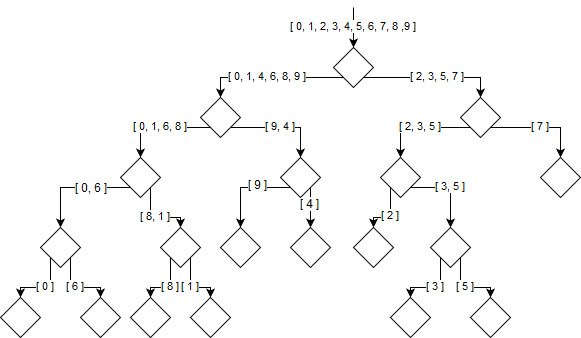
\includegraphics[width=0.8\textwidth]{Figures/balanced_tree_structure.jpg}
	\caption{Balanced Tree structure obtained during real life tests}
	\label{balanced_tree_structure}\vspace{-3pt}
\end{figure}

\subsection{Classifiers creation}

After finishing Balanced Tree architecture creation each non-leaf node is assigned a binary classifier trained on a data consisting of a training samples from classes assigned to this particular node. Those classes that are represented by its left child node are joined together and treated as a class '0', while the ones in the right child node are labelled as a class '1'. For example, if there are four classes assigned to a certain tree node, labelled as $a, b, c, d$, and a clustering method divided them into two sets $a, d$ (assigned to left child node) and $b, c$ (assigned to right child node), the classifier will be trained on data samples treating points from classes $a, d$ as if they all were from an artificial class '0' and classes $b, c$ as class '1'. The only issue that arises from such attitude is inability for leaf nodes to have their own classifiers. This is due to leafs being the last nodes in a tree, having no child nodes. To circumvent this shortcoming a solution is proposed that treats leaf node as if it had left child with the same assigned class as a parent, and a right child with assigned every existing class in the training dataset except for the class assigned to its sibling (left child node).

\subsection{Classification rules}

When an unknown, new pattern is presented to the Balanced Tree, it traverses a path from a root to a leaf node in order to be classified or rejected. This path strongly depends on classifiers in each node and their classification decision. As it was described earlier each node is assigned certain number of classes that it represents. The main task of each node's classifier is to decide if the provided pattern belongs to internal class '0' or '1'. In other words it tries to determine to which set of classes this unknown elements is most similar to. After decision is taken the patterns is sent further to the left child node in case it was classified as '0' or right one if classified as '1'. Each subsequent classifier is more precise and better clarifies pattern's class affiliation. After reaching leaf node the final classification test is made. The classifier in a leaf node is trained in an one-versus-all manner. If the unknown element is recognized as a member of a class assigned to this particular leaf, it is finally labelled as an element from that class. On the other hand if it is classified as a "rest" pattern, it gets rejected. The scheme for this approach can be seen on Figure \ref{balanced_tree_rejection}. Rejection relies on the assumption that if the pattern traversed path all way down to the leaf node, while being sent to next nodes basing on increasingly strict classifiers' decisions, and ends up being recognized as a point from outside of most probable class (the one assigned to the leaf node), then it probably is not similar enough to any class from the training set.

\begin{figure}[htp]
	\centering
	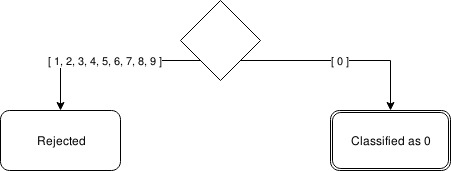
\includegraphics[width=0.6\textwidth]{Figures/balanced_tree_rejection.jpg}
	\caption{Balanced Tree rejection scheme in leaf node}
	\label{balanced_tree_rejection}\vspace{-3pt}
\end{figure}

\subsection{Implementation details}

Creation of Balanced Tree structure starts from tree root and is done recursively. Each node, that is not a tree leaf, is assigned certain set of classes which is a subset of all classes in a tree (root node is assigned all). The next step involves clustering method dividing node's class set into two disjoint sets. This procedure is done on 'class central points' which are average points of all elements in each class. Clustering algorithm divides those points thus providing two new sets for both child nodes. After that node trains its classifier on data set consisting of two classes created by taking all elements from training data for left and right child nodes' classes sets. The node-creation procedure is then applied for both node's children. The leaf creation algorithm is slightly different as it does not need usage of clustering. Classifier is trained on data set created from combining elements from training data that belongs to the same class the leaf node represents (those points' new class is labelled '0') and elements from every other class (which are labelled '1')\label{balanced_tree:one-vs-rest}. To ensure that both '0' and '1' classes have the same number of entries the '1' class set must be trimmed. This is done at its creation step by taking less elements from each class in order to have the same number (or nearly identical) of elements overall in the whole set, e.g. having training data set consisting of ten classes labelled from '0' to '9', with total of 10,000 elements, set '0' for leaf representing class '2' will have 1,000 entries of elements from class '2' taken from training data and set '1' will have 999 elements in total but will consist of elements from classes '0', '1', '3', '4', '5', '6', '7', '8', '9' taken from training data with 111 elements from each class.

\section{Slanting Tree}

\label{slanting_tree_description}

\subsection{Structure}

The Slanting Tree structure differs greatly from Balanced Tree's one. The concept implemented in Slanting Tree assumes that the unknown pattern, that is sent for classification, should be iteratively compared against each class representatives. Only when it is similar enough to points from certain class, more precise tests are made that ensure its affiliation. Should the tests fail, the pattern continues its iteration over other classes as if wasn't ever supposed to belong to this class. Rejection occurs when every test fails.

Construction of the Slanting Tree is fairly simple, unlike the Balanced Tree. Each node represents exactly one class. Nodes are chained together in such manner that when traversing Slanting Tree from the root to the last node by choosing always the left child, exactly one node for each class in the training set is visited. Each of these nodes has also a right child that can be treated as a node between its parent and its parent's left child, that extends the path received when going from root to the last node by taking always the left node's successor. Each right child node represents the same class from the training data set as its parent does.

\subsection{Classifiers creation}

Each tree node in Slanting Tree has its own binary classifier, trained in a 'one-versus-rest' manner. Training is done on data containing two classes, where the first one consists of patterns from the training set which belong to the same class as the node represents, and the second one is obtained by concatenating patterns of each class from the training set except for the class represented by the node. To prevent the situation in which node and its right child have the classifier trained on the same data (because both nodes represent the same class) certain changes to training patterns must be introduced. This ensures that every classifier in the Slanting Tree is unique and can be used during classification procedure.


\subsection{Classification rules}

The classification starts from the root node, where the unknown pattern is tested by the first classifier and has its class affiliation checked. If the obtained result indicates that it isn't similar to the class represented by this node (gets classified as an element from the 'rest' class), the classification process is continued in the next node, which is the left child of the current one. If the opposite situation occurs, and the classifier accepts presented pattern as a representative of current node's class, the process is repeated in the right child node which uses more strict classifier. This is done to ensure that the unknown element, which is supposedly from the certain class, really belongs to it. If this test fails, the pattern is sent to the node as if the previous test also failed (it is sent to the left child of the current node's parent). In case of success the pattern gets successfully classified. When all tests fail (there is no more nodes to send pattern to) the element gets rejected.

\subsection{Implementation details}

\label{slanting_tree_implementation}Creation of Slanting Tree is done recursively, starting from the root node. All classes that should be distinguishable by this tree structure are sorted by their labels and stored in an array object. This object is later used during node creation method to check what classes have already been covered by previous nodes. Every non-leaf node represents only one native class and has its binary classifier trained in 'one-vs-rest' manner, the same way the tree leafs' classifiers in Balanced Tree are (see \ref{balanced_tree:one-vs-rest}). The next step involves creating left child node for the next native class in the array object that has not yet been used. In case of no classes left the function returns without creating new node. The last step consists of right child creation, which is a leaf node. Leafs in a Slanting Tree represent the same native classes their parent node did, but their classifiers, although built using same 'one-vs-rest' approach, are trained on a different data sets in order to create more accurate results. Usually trained classifier does not achieve 100\% accuracy even on a training test that was used during its creation. There are some samples from first class that get classified as elements from the second and vice versa. Such mistakes can help determine what kind of corrections can be made to the classifier. For every non-leaf node, after its classifier training, there's set of elements from the first class that were correctly recognized (those are the elements from the class this particular node is representing) and set of elements from the second class that were mistakenly recognized as elements from the first class. Those two sets are used in this node's child leaf node's classifier creation. Of course before training those two sets must be the same size, ideally having the same number of elements as two sets used in parent's classifier training. For each missing element in either of sets the new object is generated by randomly selecting one element from this set and applying normal distribution (with standard deviation 1) to all of its features in a feature vector, thus getting new sample that can be added to the set. In case of having less than certain number of elements (implementation checks for 10 or less elements) in either of sets before new point generation algorithm takes place, those sets are filled with randomly selected points from parent node's classifier training sets.

\begin{figure}[!t]
	\centering
	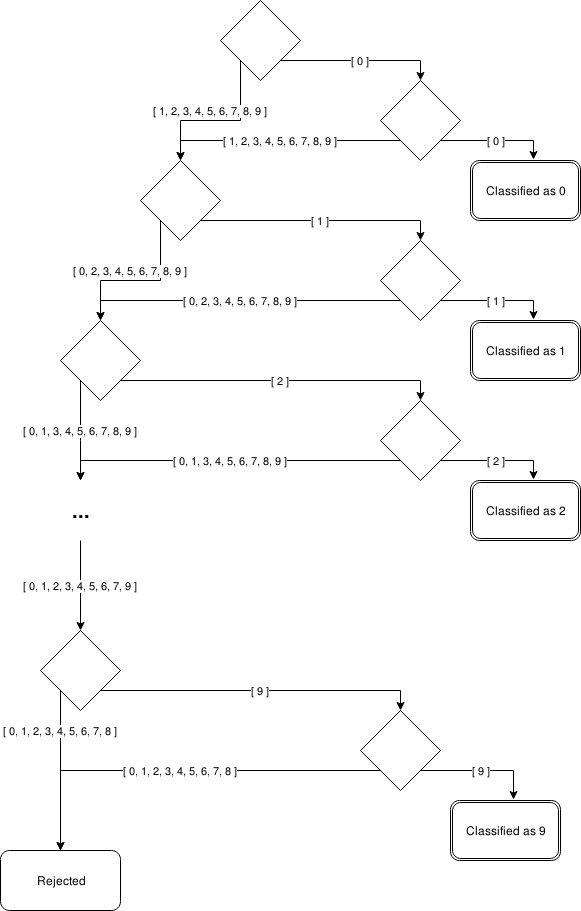
\includegraphics[width=0.7\textwidth]{Figures/slanting_tree_structure.jpg}
	\caption{Bottom part of the Slanting Tree with nodes for classes 8 and 9 (nodes for classes from 0 - 7 not visible).}
	\label{fig:rejection_version2}\vspace{-3pt}
\end{figure}

\section{Slanting Tree 2}

\subsection{Description}

Much like previously described Slanting Tree, this one has its nodes arranged in the same architecture. The difference lies in leaf nodes which, unlike the original Slanting Tree, are not using modified training data sets and use different classifier types instead (e.g. parent nodes using SVM classifier and their right children nodes using random forest). The idea behind this implementation relies on the assumption that various classifiers tend to wrongly classify different patterns, so when combining them rejection rate as well as classification rate should be vastly improved. Other than that there are no further changes and everything described in the Section \ref{slanting_tree_description} applies to Slanting Tree 2.

\subsection{Implementation details}

Creation procedure is mostly the same as in \ref{slanting_tree_implementation}. The only differences are present in nodes creation method where instead of creating new training patterns for the right child node, different classifier type is trained on the same data from the parent node.

\section{Results}

Described in this chapter classifier trees were tested with various common classifiers: SVM, kNN and random forest, using different parameters. Over 500 tests were held. Results in form of quality measurements (see Chapter \ref{quality_measures}) for training, test and letters sets were gathered in form of two matrices with 12 rows and 10 columns, one for training and one for test data. Each row in the matrix corresponds to one of the quality evaluation measurements, and each column represents value of corresponding measurement scored by certain classifier tree using one of the common classifiers. See Table \ref{example_result_matrix} for reference.

\begin{table}[htp]
	\centering
	\caption{Example empty result matrix}
	\label{example_result_matrix}
	\resizebox{\textwidth}{!}{
	\begin{tabular}{l|l|l|l|l|l|l|l|l|l|}
		\cline{2-10}
		\textbf{}                                                & \multicolumn{3}{l|}{\textbf{Balanced Tree}} & \multicolumn{3}{l|}{\textbf{Slanting Tree}} & \multicolumn{3}{l|}{\textbf{Slanting Tree 2}} \\ \cline{2-10} 
		\textbf{}                                                & \textbf{kNN}  & \textbf{SVM}  & \textbf{RF} & \textbf{kNN}  & \textbf{SVM}  & \textbf{RF} & \textbf{kNN}   & \textbf{SVM}  & \textbf{RF}  \\ \hline
		\multicolumn{1}{|l|}{\textbf{Strict Acc.}}           &               &               &             &               &               &             &                &               &              \\ \hline
		\multicolumn{1}{|l|}{\textbf{Fine Acc.}}             &               &               &             &               &               &             &                &               &              \\ \hline
		\multicolumn{1}{|l|}{\textbf{Strict Native Sens.}} &               &               &             &               &               &             &                &               &              \\ \hline
		\multicolumn{1}{|l|}{\textbf{Acc.}}                  &               &               &             &               &               &             &                &               &              \\ \hline
		\multicolumn{1}{|l|}{\textbf{Native Prec.}}          &               &               &             &               &               &             &                &               &              \\ \hline
		\multicolumn{1}{|l|}{\textbf{Native Sens.}}        &               &               &             &               &               &             &                &               &              \\ \hline
		\multicolumn{1}{|l|}{\textbf{Native F-measure}}          &               &               &             &               &               &             &                &               &              \\ \hline
		\multicolumn{1}{|l|}{\textbf{Foreign Prec.}}         &               &               &             &               &               &             &                &               &              \\ \hline
		\multicolumn{1}{|l|}{\textbf{Foreign Sens.}}       &               &               &             &               &               &             &                &               &              \\ \hline
		\multicolumn{1}{|l|}{\textbf{Foreign F-measure}}         &               &               &             &               &               &             &                &               &              \\ \hline
	\end{tabular}
	}
\end{table}

Every common classifier that was used by any of tree nodes was tested with different parameters. SVM had its C, gamma and kernel options adjusted (see Chapter \ref{common_classifiers} for every parameter explanation). Values were as follows \[ C: [ 1, 2, 4, 8, 16 ] \] \[ gamma: [ 2^{-1}, 2^{-2}, 2^{-3}, 2^{-4} ] \]  \[ kernel: [ rbf, poly ] \] 
Adjustments for kNN were made for only one parameter, using euclidean metrics \[ n\_neighbors: [ 3, 5, 7, 10 ] \]
Random forests also had modifications applied to one parameter \[ n\_estimators: [ 30, 50, 100, 150 ] \]
When evaluating results quality evaluation measurements were taken into account (see Chapter \ref{quality_measures}). Best solutions were selected by comparing $ \frac{TP + TN}{2} $ values. In the next few subsections there is short summary for each classifier tree using different internal classifiers.

\begin{table}[htp]
	\centering
	\caption{Measures values (described in Chapter \ref{quality_measures}) for classifier trees using various common classifiers on training data (described in Chapter \ref{datasets})}
	\label{classifier_trees_training_results}
	\resizebox{\textwidth}{!}{
	\begin{tabular}{l|l|l|l|l|l|l|l|l|l|}
		\cline{2-10}
		\textbf{}                                                & \multicolumn{3}{l|}{\textbf{Balanced Tree}}   & \multicolumn{3}{l|}{\textbf{Slanting Tree}} & \multicolumn{3}{l|}{\textbf{Slanting Tree 2}} \\ \cline{2-10} 
		\textbf{}                                                & \textbf{kNN}     & \textbf{SVM} & \textbf{RF} & \textbf{kNN}  & \textbf{SVM}  & \textbf{RF} & \textbf{kNN}   & \textbf{SVM}  & \textbf{RF}  \\ \hline
		\multicolumn{1}{|l|}{\textbf{Strict Acc.}}           & 20.67 & 44.92        & 41.47       & 22.76         & 29.70         & 50.29       & 38.34          & 41.51         & 40.59        \\ \hline
		\multicolumn{1}{|l|}{\textbf{Fine Acc.}}             & 92.66 & 99.33        & 100.00      & 90.61         & 91.79         & 92.43       & 94.08          & 95.41         & 95.94        \\ \hline
		\multicolumn{1}{|l|}{\textbf{Strict Native Sens.}} & 92.64 & 99.09        & 100.00      & 90.00         & 91.73         & 92.43       & 93.06          & 95.26         & 95.79        \\ \hline
		\multicolumn{1}{|l|}{\textbf{Acc.}}                  & 22.21 & 45.06        & 41.47       & 24.72         & 31.42         & 51.88       & 39.57          & 42.47         & 41.44        \\ \hline
		\multicolumn{1}{|l|}{\textbf{Native Prec.}}          & 21.23 & 27.60        & 26.38       & 21.70         & 23.41         & 30.35       & 25.62          & 26.69         & 26.35        \\ \hline
		\multicolumn{1}{|l|}{\textbf{Native Sens.}}        & 99.99 & 99.76        & 100.00      & 99.33         & 99.93         & 100.00      & 98.91          & 99.84         & 99.84        \\ \hline
		\multicolumn{1}{|l|}{\textbf{Native F-measure}}          & 35.02 & 43.23        & 41.74       & 35.62         & 37.93         & 46.57       & 40.70          & 42.13         & 41.69        \\ \hline
		\multicolumn{1}{|l|}{\textbf{Foreign Prec.}}         & 99.76 & 99.79        & 100.00      & 96.51         & 99.86         & 100.00      & 98.81          & 99.85         & 99.84        \\ \hline
		\multicolumn{1}{|l|}{\textbf{Foreign Sens.}}       & 1.58 & 30.55        & 25.94       & 4.92          & 13.25         & 39.11       & 23.82          & 27.25         & 25.94        \\ \hline
		\multicolumn{1}{|l|}{\textbf{Foreign F-measure}}         & 3.10  & 46.78        & 41.20       & 9.37          & 23.39         & 56.23       & 38.39          & 42.82         & 41.18        \\ \hline
	\end{tabular}
	}
\end{table}

\begin{table}[htp]
	\centering
	\caption{Measures values (described in Chapter \ref{quality_measures}) for classifier trees using various common classifiers on test data (described in Chapter \ref{datasets})}
	\label{classifier_trees_test_results}
	\resizebox{\textwidth}{!}{
		\begin{tabular}{l|l|l|l|l|l|l|l|l|l|}
			\cline{2-10}
			\textbf{}                                                & \multicolumn{3}{l|}{\textbf{Balanced Tree}} & \multicolumn{3}{l|}{\textbf{Slanting Tree}} & \multicolumn{3}{l|}{\textbf{Slanting Tree 2}} \\ \cline{2-10} 
			\textbf{}                                                & \textbf{kNN}  & \textbf{SVM}  & \textbf{RF} & \textbf{kNN}  & \textbf{SVM}  & \textbf{RF} & \textbf{kNN}   & \textbf{SVM}  & \textbf{RF}  \\ \hline
			\multicolumn{1}{|l|}{\textbf{Strict Acc.}}           & 10.79         & 37.04         & 32.81       & 13.41         & 21.18         & 44.21       & 30.72          & 33.94         & 32.75        \\ \hline
			\multicolumn{1}{|l|}{\textbf{Fine Acc.}}             & 91.86         & 96.44         & 95.56       & 88.89         & 91.49         & 90.36       & 93.45          & 95.02         & 94.56        \\ \hline
			\multicolumn{1}{|l|}{\textbf{Strict Native Sens.}} & 91.77         & 94.03         & 93.23       & 88.00         & 90.97         & 89.03       & 91.33          & 92.80         & 92.67        \\ \hline
			\multicolumn{1}{|l|}{\textbf{Acc.}}                  & 11.62         & 37.39         & 33.26       & 14.53         & 22.05         & 45.18       & 31.37          & 34.44         & 33.30        \\ \hline
			\multicolumn{1}{|l|}{\textbf{Native Prec.}}          & 10.35         & 13.77         & 13.03       & 10.59         & 11.53         & 15.54       & 12.73          & 13.24         & 13.08        \\ \hline
			\multicolumn{1}{|l|}{\textbf{Native Sens.}}        & 99.90         & 97.50         & 97.57       & 99.00         & 99.43         & 98.53       & 97.73          & 97.67         & 98.00        \\ \hline
			\multicolumn{1}{|l|}{\textbf{Native F-measure}}          & 18.75         & 24.13         & 22.99       & 19.13         & 20.66         & 26.85       & 22.53          & 23.33         & 23.08        \\ \hline
			\multicolumn{1}{|l|}{\textbf{Foreign Prec.}}         & 99.28         & 99.08         & 98.94       & 97.74         & 99.52         & 99.58       & 98.93          & 99.04         & 99.13        \\ \hline
			\multicolumn{1}{|l|}{\textbf{Foreign Sens.}}       & 1.58          & 30.55         & 25.94       & 4.92          & 13.25         & 39.11       & 23.82          & 27.25         & 25.94        \\ \hline
			\multicolumn{1}{|l|}{\textbf{Foreign F-measure}}         & 3.10          & 46.70         & 41.11       & 9.38          & 23.38         & 56.16       & 38.40          & 42.74         & 41.12        \\ \hline
		\end{tabular}
	}
\end{table}

\subsection{Balanced Tree}

\subsubsection{SVM}

The best results for Balanced tree with SVM classifier are achieved when using polynomial kernel, gamma 0.5 and C parameter value of 16. Generally, for polynomial kernel, better results are achieved when using bigger C values (gamma doesn't have as much impact). Similar conclusion can also be made for rbf kernel, which performs only slightly worse than the polynomial one.

\subsubsection{Random Forests}

When using random forest as its classifier the Balanced Tree doesn't improve much. Whereas more native patterns are correctly recognized and assigned their labels, the foreign patterns aren't properly rejected. As it can be seen in the result Tables \ref{classifier_trees_training_results} and \ref{classifier_trees_test_results} Balanced Tree using random forest displays tendency to classify unknown pattern rather than reject it. The presented score was achieved while using random forest classifier with 30 estimators.

\subsubsection{k-Nearest Neighbours}

Unfortunately using kNN classifier doesn't bring any positive changes. Rejection mechanism is almost non-existent and the native pattern classification isn't satisfying. The best results are achieved when using 10 nearest neighbours to determine point affiliation.

\subsection{Slanting Tree}

\subsubsection{SVM}

Unlike Balanced tree using SVM, where either kernel parameter value yields similar results, Slanting Tree works best when using rbf kernel. Bigger gamma values also help maintaining higher foreign patterns rejection rates, although the final results are worse than those achieved by Balanced tree.

\subsubsection{Random Forests}

Slanting Tree performs best when using random forest as its internal classifier. Although it presents excellent classification abilities and the rejection rate is best among all classifier trees tested, it still can be considered only mediocre in terms of usefulness. The results, which are contained within Tables \ref{classifier_trees_training_results} and \ref{classifier_trees_test_results}, were obtained when using 100 estimators for each random forest classifier.

\subsubsection{k-Nearest Neighbours}

Similarly to Balanced tree, using kNN classifier in Slanting Tree does not work as expected. Not only its classification is bad but also rejection does not bring satisfying results, even when using kNN classifiers that takes into consideration only 2 nearest neighbours for each presented, unknown pattern.


\subsection{Slanting Tree 2}

\subsubsection{SVM}

Bigger C value again proves to be better when using SVM classifier. Similarly to Balanced Tree, using either polynomial or rbf kernel doesn't have much impact on the final results. This time it is the second common classifier that played crucial part in attaining results presented in Tables \ref{classifier_trees_training_results} and \ref{classifier_trees_test_results}. In every case, when using random forest, both classification and rejection rates are very high, with 30 estimators performing the best.

\subsubsection{Random Forests}

When using random forest as its main classifier, the Slanting Tree 2 scores best result with SVM as the second common classifier. The main similarity between best solution obtained for Slanting Tree 2 using SVM as its main common classifier and the one using random forest is that both of them use in fact the same two classifiers but in a reversed order. After comparing results in both Tables \ref{classifier_trees_training_results} and \ref{classifier_trees_test_results} it can be seen that for Slanting Tree 2 it's better to use SVM backed up by random forests as its rejection rate is higher.

\subsubsection{k-Nearest Neighbours}

Unlike the original Slanting Tree, the version 2 does perform well when using kNN. After adding random forest as the second common classifier the rejection rate has increased almost 5 times. Despite the changes, the obtained solution is still outperformed by previous Slanting Tree constructions (most notably the one using SVM and random forest combination) which questions its usefulness. 

\section{Summary}

All of the classifier trees introduced in this chapter had good classification capabilities, very similar to the plain common classifiers they used. It is worth noting that not only did the classification rate stayed the same, but also rejection capabilities were introduced. Among all classifiers combinations tested it was the Slanting tree using random forests with 100 estimators that performed the best. Tables \ref{classifier_trees_training_results} and \ref{classifier_trees_test_results} show score achieved by this tree structure. Although being the best, classification rate achieved by this particular Slanting Tree may not be considered good, as it's lower than 50\%. At best it could be seen as mediocre. Despite trying different classifiers and their parameters combinations no better solution could be found while using tree structures described in this chapter. The final conclusion can be made that the classifier trees introduced in this paper do not perform well enough to be used as a valid rejection mechanism. While still maintaining high classification rates those structures are slower than other popular classifiers which questions their usefulness. % Experimental Setup

%\input{Chapters/Chapter4} % Experiment 1

%\input{Chapters/Chapter5} % Experiment 2

%\input{Chapters/Chapter6} % Results and Discussion

%\input{Chapters/Chapter7} % Conclusion

%% ----------------------------------------------------------------
% Now begin the Appendices, including them as separate files

\addtocontents{toc}{\vspace{2em}} % Add a gap in the Contents, for aesthetics

\appendix % Cue to tell LaTeX that the following 'chapters' are Appendices

\lhead{\emph{An Appendix}}
\chapter{An Appendix}
	% Appendix Title

%\input{Appendices/AppendixB} % Appendix Title

%\input{Appendices/AppendixC} % Appendix Title

\addtocontents{toc}{\vspace{2em}}  % Add a gap in the Contents, for aesthetics
\backmatter

%% ----------------------------------------------------------------
\label{Bibliography}
\lhead{\emph{Bibliography}}  % Change the left side page header to "Bibliography"
\bibliographystyle{unsrtnat}  % Use the "unsrtnat" BibTeX style for formatting the Bibliography
\bibliography{Bibliography}  % The references (bibliography) information are stored in the file named "Bibliography.bib"

\end{document}  % The End
%% ----------------------------------------------------------------